\documentclass{article}

\usepackage{url}
\usepackage{biblatex}
\usepackage{graphicx}
\usepackage[usenames]{color}
\usepackage{tikz}

\definecolor{red}{rgb}{1, 0, 0}

\bibliography{project_milestone.bib}

\title{Project Report - CSE 590 Fall 2012}
\author{Anirban Mitra\\
anmitra@cs.stonybrook.edu\\
Stony Brook ID: 108672767}

\begin{document}
    \maketitle
    \section{Introduction}
        The abundance of data has given rise to the art of mining data itself to get relevant and meaningful insights. A large class of this {\em BigData} can be modeled as graph and useful results can be inferred just from the structure of the graph. For example, recommendation system for products can be modelled as bipartite graph of users and products and we can recommend a user the products that many of his/her friends has bought in recent past. Similarly, problems like fraud detection, disease prevention, climate change etc are being attacked using such methods of graph analysis. The scale of {\em BigData} itself poses a engineering challenge. Here, distributed systems like {\em Hadoop} using {\em MapReduce} programming paradigm have become popular as solution.
        
        But, the scale of {\em big data} is not the only challenge. On top of that, answering {\em NP-complete} or {\em NP-hard} problems about a given graph frequently come up. These questions are often part of larger practical graph problems that are interesting to us. A possible solution is to turn our attention to good approximate answers to such {\em hard problems}. Recently, {\em graph coordinate systems} like Orion \cite{Orion} have been proposed, inspired from network coordinate system \cite{Vivaldi}, to map nodes in graph to points in plane which can provide accurate and efficient solutions to such hard queries.
        
    \section{Motivation}
    
        With {\em graph coordinate systems} we can leverage a host of geometric algorithms developed for points in a plane problems for solving the corresponding {\em hard graph problems}. Thus we will be able to have good approximate polynomial time solutions {\em NP-complete} or {\em NP-hard} graph problems. The focus of this project will be to try to solve the {\em Community Detection} problems in a graph using the algorithms for the {\em Minimum N-Disk Problem}. Since we are now able to map graph nodes to points in a plane using {\em graph coordinate systems} like \cite{Vivaldi}.
        
    \section{Definitions}
        
        \subsection{Minimum N-Disk Problem}
            {\em Given $N$ points in a plane, what the minimum radius circle which contains all the $N$ points.} \\
        
        If we apply the algorithm for this problem on the the {\em graph coordinates} of the complete graph then it should give us a good approximate diameter of the graph. But, in this project, we will be explore the solution of the following problem
        
        \subsection{Dense Community Problem}
            {\em Given a community diameter $d$, which is the largest subgraph such that its diameter is at most $d$.} \\
        
        The algorithm presented in \cite{Efrat99} can be adapted to solve the {\em Dense Community Problem}. The above problem contains the following as a subproblem
        
        \subsection{Dense Community Membership Problem}
            {\em Given a diameter $d$ and node $v$, which is the largest subgraph with its diameter at most $d$ and containing $v$.} \\
        
        The algorithm will be adapted to {\em MapReduce} paradigm so that we can use {\em Hadoop} as a platform to apply this on very large graph coordinates with  time complexity given a diameter $d$.
    
    \section{Algorithm}
    
    \subsection{Circle passing through three points (Naive method)}

        It is clear that there can be many candidates for the smallest circle containing $N$ or more points. But also, all of the smallest circles will have 2 or more points on its circumference. Lets prove this using a thought experiment.

        Let us assume that we know the any one of the smallest circle and the corresponding set of $N$ points. Ignore all other points. It is clear that the smallest circle for this given set will be unique. Start with an arbitrary large circle containing all the $N$ points. Now, go on shrinking the circle till one or more of the points lie on its circumference. If there is only one point on the circumference, then rotate the circle about the point (in either direction) till another point lies on the circumference. So, in either cases, we will end up with a circle with two points on the circumference.

        If the points on the circumference are diametrically opposite then this is the smallest circle because any smaller circle can not contain both the points. So, in this case the smallest circle has two points on the circumference.

        Else, let $L$ be the line segment joining the points on the circumference and $M$ be the perpendicular bisector as shown in Figure 1. We will further shrink the circle by moving the centre towards $L$ along $M$ till either another point lies on the circumference or the $L$ becomes a diameter. In either case, no smaller circle containing all the points is possible, hence it is the smallest circle and it has 2 or more points on its circumference. Hence the result is proved. \\

        \begin{figure}
            \centering
            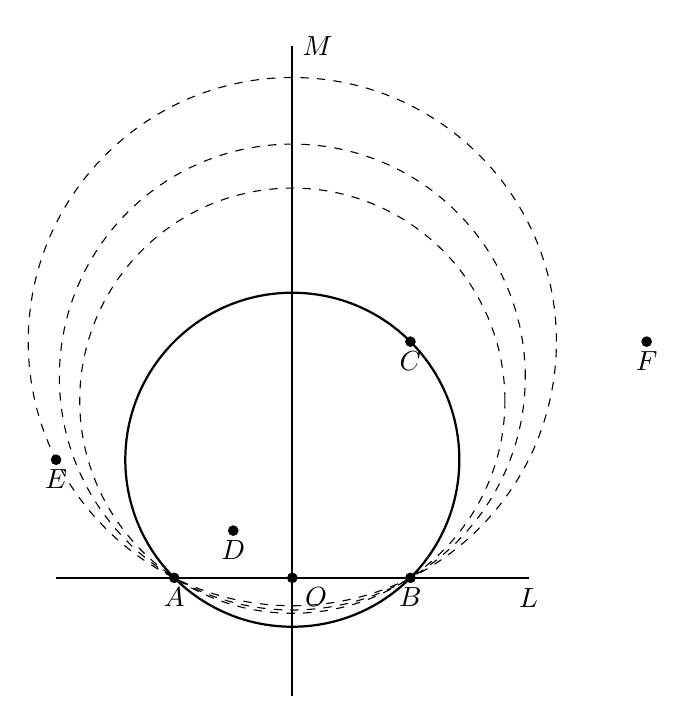
\begin{tikzpicture}[scale=1.5]
                \draw[thick] (-2, 0) -- (2, 0) node[right, below] {$L$};
                \draw[thick] (0, -1) -- (0, 4.5) node[right] {$M$};
                \draw[fill=black] (0, 0) circle (.04cm) node[right=.3cm, below] (origin) {$O$};
                \draw[fill=black] (-1, 0) circle (.04cm) node[below] (A) {$A$};
                \draw[fill=black] (1, 0) circle (.04cm) node[below] (B) {$B$};
                \draw[fill=black] (1, 2) circle (.04cm) node[below] (C) {$C$};
                \draw[fill=black] (-.5, .4) circle (.04cm) node[below] (D) {$D$};
                \draw[fill=black] (-2, 1) circle (.04cm) node[below] (E) {$E$};
                \draw[fill=black] (3, 2) circle (.04cm) node[below] (F) {$F$};
                \draw[dashed] (0, 2) circle (2.236cm);
                \draw[dashed] (0, 1.7) circle (1.9723cm);
                \draw[dashed] (0, 1.5) circle (1.8cm);
                \draw[thick] (0, 1) circle (1.414cm);
            \end{tikzpicture}
            \caption {Smallest circle containing $N=4$ points}
        \end{figure}

        Hence in the naive method, do the following steps
        \begin{enumerate}
            \item For every pair of points as diameter, draw the circle and find out the number of points contained in. Find the smallest circle among them containing N or more points, if any.
            \item For every triplet of points, draw the corresponding circumcircle and find out the smallest circle containing $N$ or more points. Find the smallest among them.
        \end{enumerate}

        The answer is the smaller one from either. Obviously, the complexity is $O(N^4)$.

        \subsection{Circle passing through two points}

        Choose any two points from the set P and Q. Now we will find the smallest circle passing through these two points and containing N points. If we can do that, then we can repeat the same for every pair of points and choose the optimal answer.

        Let the equation of the line passing through $P$ and $Q$ be $L(Z) = 0$. Hence, $L(P) = 0$ and $L(Q) = 0$. Now consider any third point $X$ (say $L(x) > 0$) and consider the angle $PXQ$. We know that for the circumcircle passing through $P$, $Q$, and $X$, any point on the circumference (on the same side of $PQ$) subtends equal angle, any point outside subtends smaller angle and points inside subtend greater angles. So, we can easily sort the points by the angles subtended at $PQ$. Now if we choose any point from the sorted sequence say $Y$, then all the points to the right of it will also be inside the circle. To include the points from the other side of $PQ$ too, consider any random point say $K$ (i.e. $L(K) < 0$ ) and

        \begin{enumerate}
            \item If $PKQ$ is equal to $(180 - PXQ)$, it lies on the circumference
            \item If $PKQ$ greater than $(180 - PXQ)$, it lies inside the circle, otherwise outside
        \end{enumerate}

        \begin{figure}
            \centering
            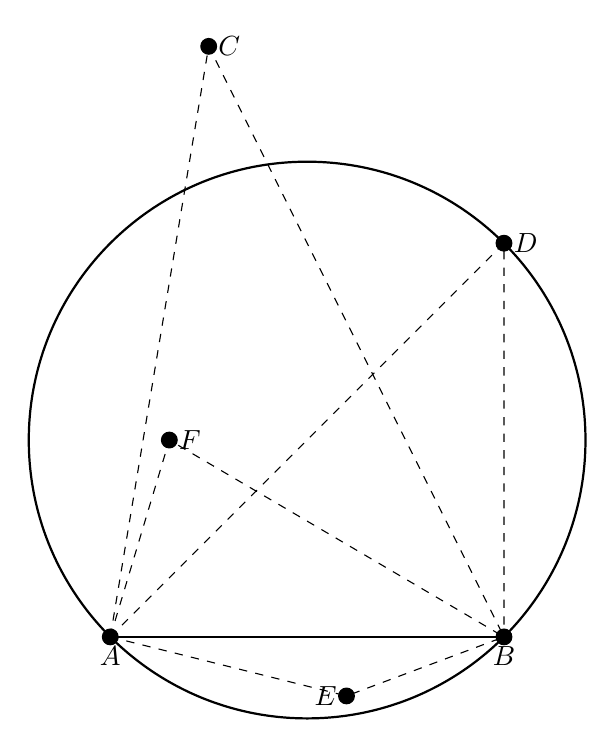
\begin{tikzpicture}[scale=2.5]
                \draw[fill=black] (-1, 0) circle (.04cm) node[below] (A) {$A$};
                \draw[fill=black] (1, 0) circle (.04cm) node[below] (B) {$B$};
                \draw[thick] (1, 0) -- (-1, 0);
                \draw[thick] (0, 1) circle (1.414cm);
                \draw[fill=black] (-.7, 1) circle (.04cm) node[right] (F) {$F$};
                \draw[fill=black] (1, 2) circle (.04cm) node[right] (D) {$D$};
                \draw[fill=black] (-.5, 3) circle (.04cm) node[right] (C) {$C$};
                \draw[fill=black] (.2, -.3) circle (.04cm) node[left] (E) {$E$};
                \draw[dashed] (-1, 0) -- (1, 2) -- (1, 0);
                \draw[dashed] (-1, 0) -- (.2, -.3) -- (1, 0);
                \draw[dashed] (-1, 0) -- (-.7, 1) -- (1, 0);
                \draw[dashed] (-1, 0) -- (-.5, 3) -- (1, 0);
            \end{tikzpicture}
            \caption {Sorted points according to the rules: $C, D, E, F$}
        \end{figure}

        To be complete, for points on PQ (i.e. $L(X) = 0$) the ones that lie between $PQ$, the they will always be inside otherwise, the others can be ignored.

        Using these together, we can sort all the points and choose the optimal third point to draw the circumcircle and calculate the radius. For one pair of points the complexity is $O(N \times log(N))$ and hence the overall complexity is $O(N^3 \times log(N))$.

        \subsection{Circle passing through one point}

        Consider all the circles of certain radius R hinged at one of the given points say $X$. The locus of centres of all such circles is a circle of radius $R$ centered at $X$. Now consider any other point in the set, say $Y$ and let it be outside the circle of locus. Drop line segments from $Y$ on the circumference of the circle ($YA$ and $YB$ as shown in the figure) such that $YA = YB = R$. Now for any circle of radius $R$ and passing through $X$, having its centre between $A$ and $B$ (including them) will contain $Y$. Since the the distance of all the points of the arc $AB$ from $Y$ is less than or equal to $R$. \\

        \begin{figure}
            \centering
            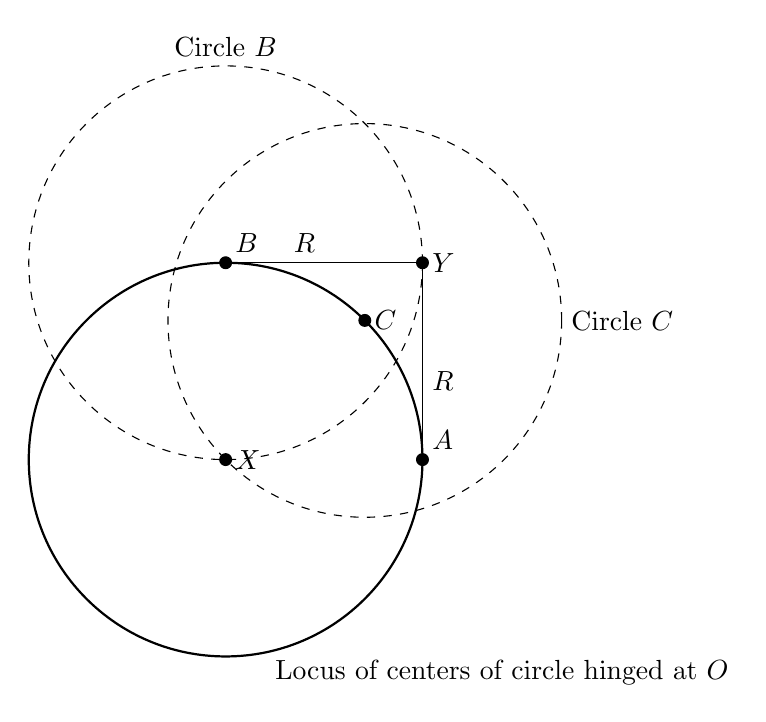
\begin{tikzpicture}[scale=2.5]
                \draw[fill=black] (0, 0cm) circle (.03cm) node[right] (X) {$X$};
                \draw[fill=black] (1, 1cm) circle (.03cm) node[right] (Y) {$Y$};
                \draw[fill=black] (1, 0cm) circle (.03cm) node[above right] (A) {$A$};
                \draw[fill=black] (0, 1cm) circle (.03cm) node[above right] (B) {$B$};
                \draw[fill=black] (.707, .707cm) circle (.03cm) node[right] (C) {$C$};
                \draw (1, 1cm) -- (1, 0cm) node[above=1cm, right] {$R$};
                \draw (1, 1cm) -- (0, 1cm) node[right=1cm, above] {$R$};
                \draw[thick] (0, 0cm) circle (1cm) node[below=2.7cm, right=.5cm] (locus) {Locus of centers of circle hinged at $O$};
                \draw[dashed] (.707, .707cm) circle (1cm) node[right=2.5cm] {Circle $C$};
                \draw[dashed] (0, 1cm) circle (1cm) node[above=2.5cm] {Circle $B$};
            \end{tikzpicture}
            \caption{Both circle $A$ and $B$ contains $Y$}
        \end{figure}

        This is true for points in the set lying inside the circle of locus too. So, if we can calculate the arc intervals for all the points (other than $X$) in the set and find out where maximum number of intervals overlap, we will have the maximum points contained in a cicle of radius $R$ and passing through $X$. Algorithms are known to solve the maximum interval overlap problem in $O(N \times log(N))$ (note that the interval is circular). \\

        Now to find out the smallest circle passing through $X$ and having $N$ points, we can do a binary search on R and each time calculate the maximum points inside possible using the above method which should be greater or equal to $N$ to be a valid radius. The cost of this is $O(N \times log(N) \times log(RMAX))$ where say $RMAX$ is a suitable arbitrary large radius. And, since we will do do this for every point the total cost is $O(N^2 \times log(N) \times log(RMAX))$.
    
    \section{Dataset}
    
        The data of the ten Facebook networks provided from the {\em SNAP - Stanford Network Analysis Project} website \cite{snap} will be used for the evaluation here. Here are some interesting statistics about the data
        
        \begin{center}
            \begin{tabular}{ |l|r| }
                \hline
                Nodes & 4039 \\
                \hline
                Edges & 88234 \\
                \hline
                Average Clustering Coefficient & 0.6055 \\
                \hline
                Diameter & 8 \\
                \hline
                90-percentile Diameter & 4.7 \\
                \hline
            \end{tabular}
        \end{center}
        
        Here is the visualization of one of the ten graphs present in the data using {\em Gephi} \cite{gephi}.
        
        \begin{center}
            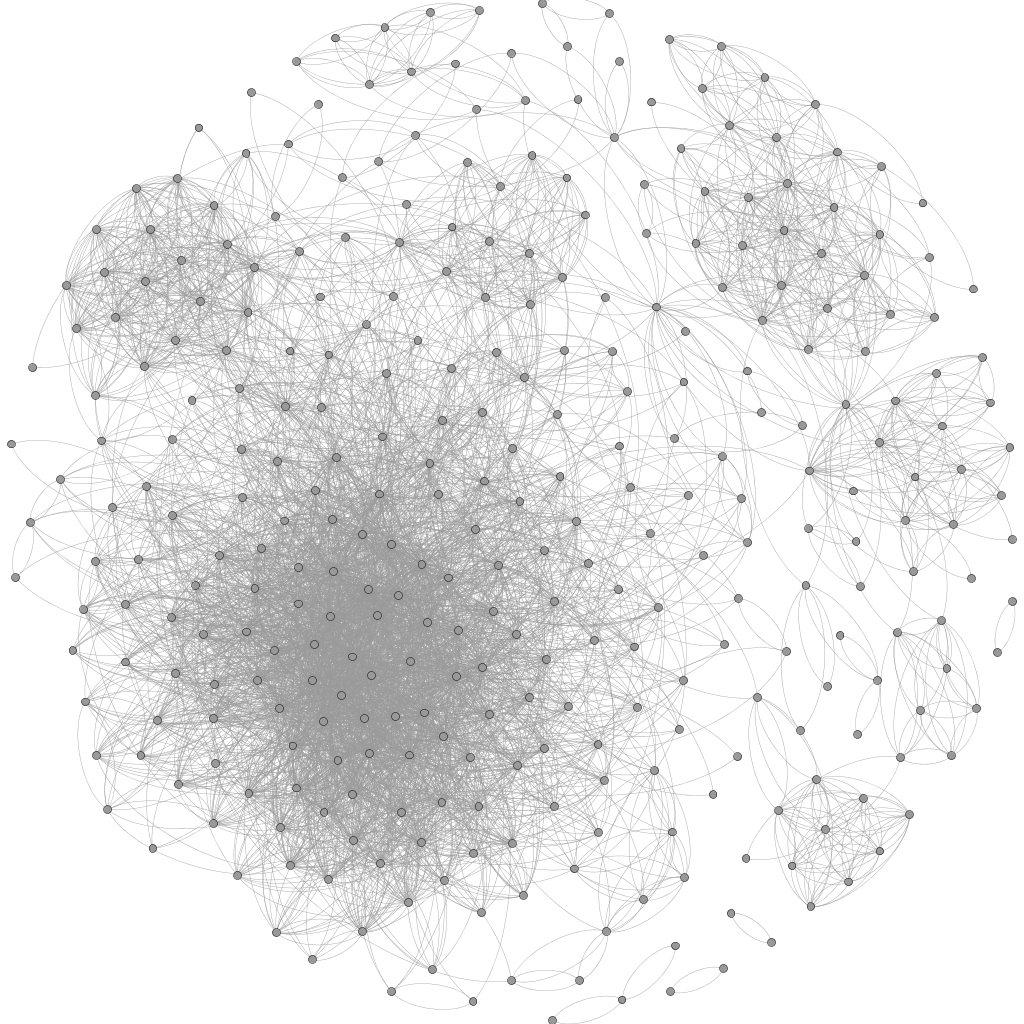
\includegraphics[scale=0.4]{fb0_graph.png}
        \end{center}
        
    \section{Results}
    
        Here is the 2D plot of graph data mapped on the plane points using {\em cmdscale} in {\em R} \cite{cmdscale}.
        
        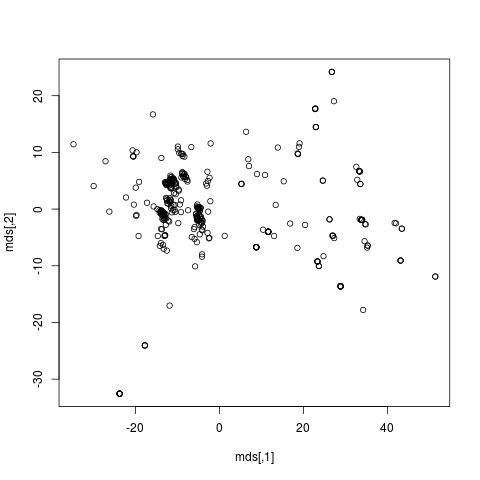
\includegraphics[scale=0.8]{fb0_2d.png}
        
        \subsection{Runtime}
        
            Here we will evaluate the runtime of the proposed {\em Dense Community Problem} with respect to the {\em brute force} implementation. This comparison will be done on random data sets of different sizes. Obviously, this will give us good estimate of the runtime when we run this on {\em graph coordinates}. Here is the table comparing the $O(n^4)$ brute force algorithm with $n^2 \log n$ algorithm.
            \begin{center}
            \begin{tabular}{| c | c | c |}
                \hline
                Size & Brute Force Time & Optimised Time \\
                \hline
                50 & 0m0.139s & 0m0.038s \\
                \hline
                100 & 0m0.750s & 0m0.129s \\
                \hline
                200 & 0m11.127s & 0m0.493s \\
                \hline
                500 & 17m12.904 & 0m3.185s \\
                \hline
                1000 & & 0m13.252s \\
                \hline
                2000 & & 0m56.208s \\
                \hline
                5000 & & 6m34.802s \\
                \hline
            \end{tabular}
            
            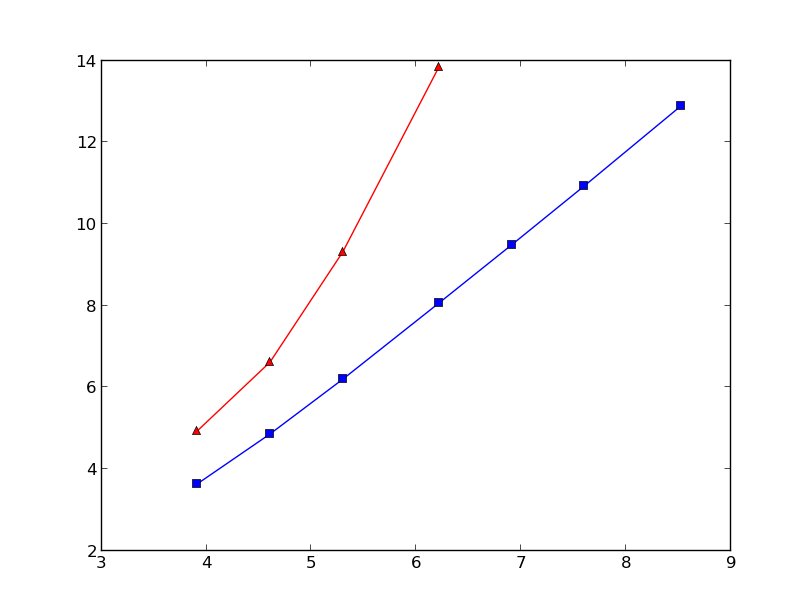
\includegraphics[scale=0.8]{runtime.png}
            \end{center}
            As it is clear from the  table that the $n^2 \log n$ algorithm runs much better for large and large datasets.
        
        \subsection{All Pair Distances}
        
            Here we will compare the variation of the distances between any two nodes in the original graph and the {\em graph coordinates}. For a good approximation the variations of the all pairwise distances in the two instances should match with each other.
            
            This first graph shows the variation of top thousand pair distances in the actual graph and the graph coordinates.
            
            \noindent 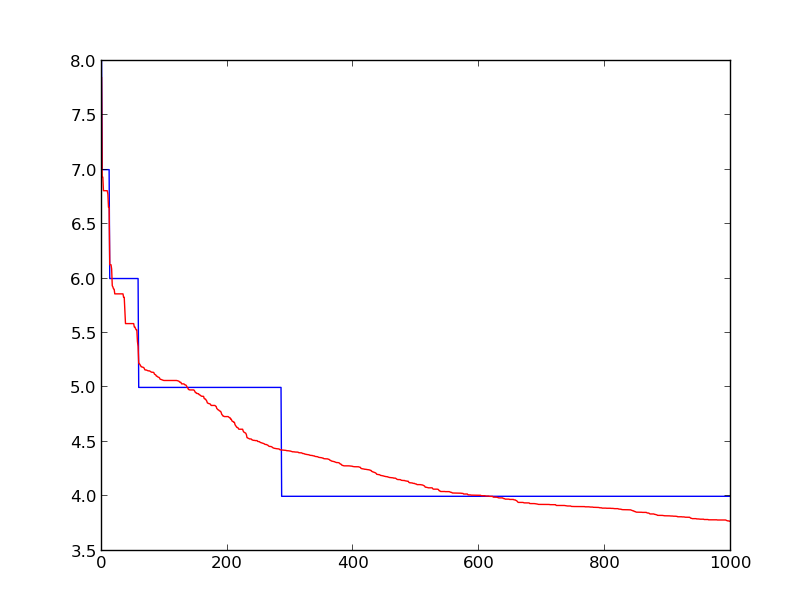
\includegraphics[scale=0.8]{pairs_top_1000.png}
            
            Here is the comparison for all the pairs.
            
            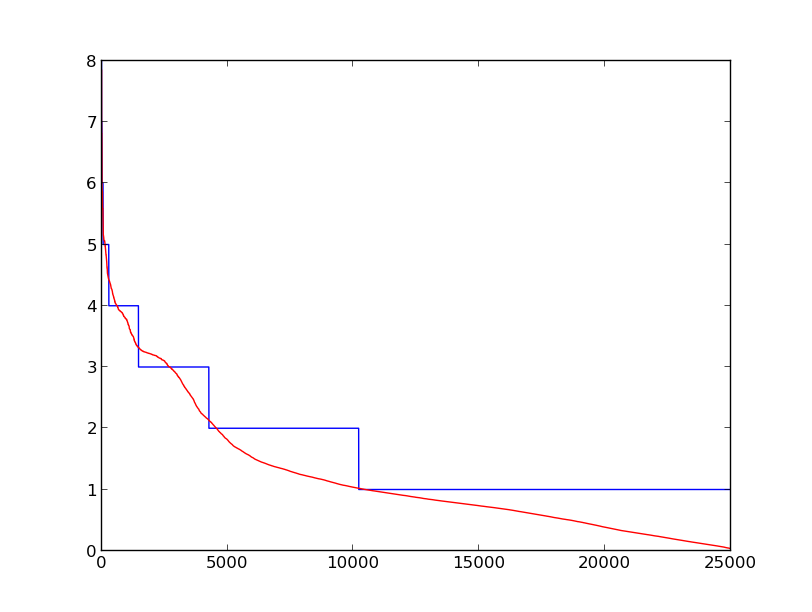
\includegraphics[scale=0.8]{total_pairs.png}
            
            
            It is inferred that the variation of distances between pairs in the graph coordinate systems fits nicely with the actual values.
            
        \subsection{Diameter}
            
            If we use the solution for the {\em Dense Community Problem} and do a binary search on the on the diameter value {\em d}, we can easily find out the diameter of the graph. The intention here is to evaluate how well we are able to estimate the diameter of the graph using {\em graph coordinates} and the {\em Dense Community Problem} algorithm. This is a way to validate our approach to get an approximate solution of the diameter.
            
            Here is the graph comparing the actual diameter with the graph coordinate diameter for different sets of data.
            
            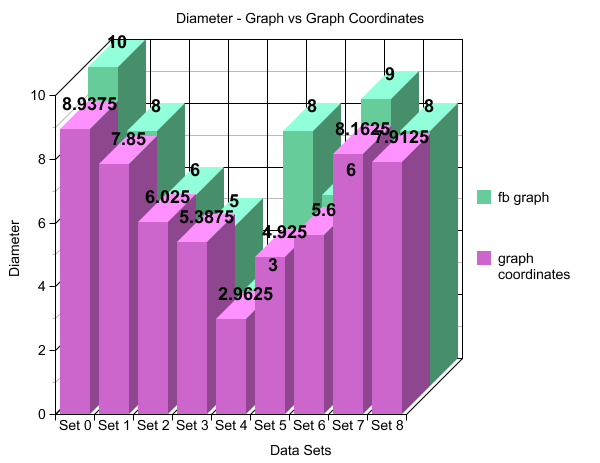
\includegraphics[scale=0.8]{diameter.png}
            
    \section{Conclusion}
    
        For many purposes, like estimation of distance between two nodes or estimation of diameter of graph, can be very easily and quite accurately done using the graph coordinate system. Also, many NP-complete graph problems reduces to small polynomial time geometric algorithm with good approximate algorithms. As, part of further work, it can be easily seen that presented algorithm can be used to partition the graph into communities too.
            
    \section{Code}
    
        The code that I wrote for the project can be found on {\em Github} at \url{https://github.com/nomind/DataMiningFall2012}.
        
    \section{References}
     
        \printbibliography
    
\end{document}


